\documentclass[tikz,border=4pt]{standalone}
\usepackage[T1]{fontenc}
\usepackage[utf8]{inputenc}
\usepackage{FiraSans}
\usepackage{amsmath}
\usetikzlibrary{arrows.meta,positioning,calc}
\definecolor{ceBlue}{RGB}{42,96,153}
\definecolor{ceTeal}{RGB}{36,135,118}
\definecolor{ceGold}{RGB}{220,160,52}
\definecolor{ceRed}{RGB}{188,74,60}
\definecolor{ceInk}{RGB}{42,42,42}
\definecolor{ceGray}{RGB}{238,240,242}
\begin{document}
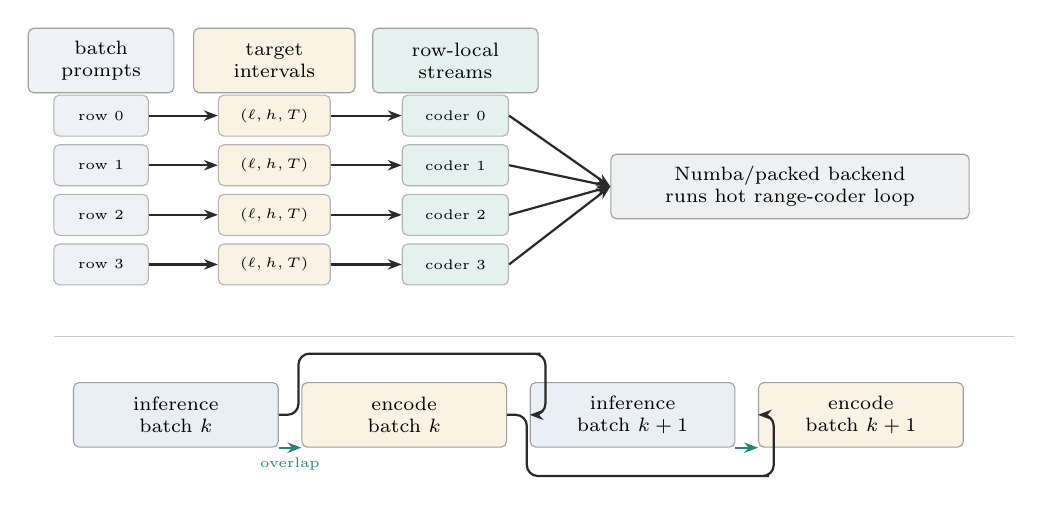
\begin{tikzpicture}[
  x=1cm,y=1cm,
  font=\sffamily,
  row/.style={draw=ceInk!35, rounded corners=2pt, fill=white, minimum width=1.2cm, minimum height=0.52cm, font=\tiny},
  work/.style={draw=ceInk!45, rounded corners=2pt, align=center, font=\scriptsize, minimum height=0.82cm},
  arr/.style={-{Stealth[length=5pt]}, thick, ceInk},
]
  \foreach \r/\y in {0/5.35,1/4.72,2/4.09,3/3.46} {
    \node[row, fill=ceBlue!8] (p\r) at (1.15,\y) {row \r};
    \node[row, fill=ceGold!14, minimum width=1.42cm] (i\r) at (3.35,\y) {$(\ell,h,T)$};
    \node[row, fill=ceTeal!12, minimum width=1.35cm] (c\r) at (5.65,\y) {coder \r};
    \draw[arr] (p\r) -- (i\r);
    \draw[arr] (i\r) -- (c\r);
  }
  \node[work, fill=ceBlue!8, minimum width=1.85cm] at (1.15,6.05) {batch\\prompts};
  \node[work, fill=ceGold!14, minimum width=2.05cm] at (3.35,6.05) {target\\intervals};
  \node[work, fill=ceTeal!12, minimum width=2.1cm] at (5.65,6.05) {row-local\\streams};

  \node[work, fill=ceGray, minimum width=4.55cm] (cpu) at (9.9,4.45) {Numba/packed backend\\runs hot range-coder loop};
  \foreach \r in {0,1,2,3} {
    \draw[arr] (c\r.east) -- (cpu.west);
  }

  \draw[ceInk!25] (0.55,2.55) -- (12.75,2.55);
  \node[work, fill=ceBlue!10, minimum width=2.6cm] (inf0) at (2.1,1.55) {inference\\batch $k$};
  \node[work, fill=ceGold!14, minimum width=2.6cm] (enc0) at (5.0,1.55) {encode\\batch $k$};
  \node[work, fill=ceBlue!10, minimum width=2.6cm] (inf1) at (7.9,1.55) {inference\\batch $k+1$};
  \node[work, fill=ceGold!14, minimum width=2.6cm] (enc1) at (10.8,1.55) {encode\\batch $k+1$};
  \draw[arr, rounded corners=4pt]
    (inf0.east) -- ++(0.25,0) |- ([yshift=0.36cm]inf1.north west) -- ++(0.2,0) |- (inf1.west);
  \draw[arr, rounded corners=4pt]
    (enc0.east) -- ++(0.25,0) |- ([yshift=-0.36cm]enc1.south west) -- ++(0.2,0) |- (enc1.west);
  \draw[arr, ceTeal] (inf0.south east) -- node[below, font=\tiny, ceTeal] {overlap} (enc0.south west);
  \draw[arr, ceTeal] (inf1.south east) -- (enc1.south west);
\end{tikzpicture}
\end{document}
